% !TeX encoding = ISO-8859-1
\chapter{Solución exacta}
\label{cha:primera}


En este capítulo calcularemos las soluciones tipo solitón de nuestra ecuación BBMB (\ref{ec_1}).

\section{Marco teórico}

Vamos a definir algunos conceptos previos necesarios para la la obtención de soluciones tipo solitón de nuestra ecuación, la cual es una EDP no lineal.

\subsection{Ondas viajeras}

Una onda viajera es una onda que recorre grandes distancias y se desplaza libremente por el medio, transfiriendo energía sin propagación de la materia. De forma matemática se define como sigue:

\begin{definicion1}[label={definicion1},nameref={Title or anything else}]{Onda viajera}
    \textit{Una onda viajera es una función que mantiene su forma durante largos periodos de tiempo, la cual viene dada por:}
$$u(x,t)=f(x-ct),$$
\textit{donde $c$ representa la velocidad de la onda.}
\end{definicion1}\label{ondaviajera}

Podemos observar que para el instante $t=0$, la onda tiene la forma de la condición inicial $f(x)$, también llamado perfil de la onda. Por tanto, dado un instante de tiempo $t>0$, obtendremos $f(x-ct)$, que representa el valor en el tiempo $t$, la cual es la condición inicial trasladada a la derecha $ct$ unidades sin deformarse con velocidad $c>0$. De forma análoga, dada $c<0$, obtendremos  $f(x+ct)$, que es la condición inicial trasladada a la izquierda $ct$ unidades sin deformarse con velocidad $c$. \\

La resolución de EDPs no lineales suele ser bastante compleja, por lo que en este trabajo vamos a centrarnos en la búsqueda de soluciones tipo onda viajera, en concreto onda solitaria de tipo solitón, ya que tiene notables aplicaciones físicas. A continuación introducimos el concepto de onda solitaria.

\subsection{Onda solitaria}

\begin{definicion1}[label={definicion},nameref={Title or anything else}]{Onda solitaria}
    \textit{Se denomina onda solitaria a aquella onda viajera no lineal localizada espacialmente y estable, además de ``suave", esto es:}
$$ u(x,t) \rightarrow 0 \quad \mbox{cuando} \quad x \rightarrow \pm \infty $$
\textit{donde $c$ representa la velocidad de la onda.}
\end{definicion1}


\subsection{Solitón}


Habitualmente, cuando dos ondas solitarias no lineales con diferentes velocidades interactúan, cambian su forma o adquieren colas. Por el contrario, cuando dos ondas solitarias mantienen su forma y velocidad después de la interacción, se les denomina solitones.

\begin{definicion1}[label={definicion},nameref={Title or anything else}]{Solitón}
    \textit{Los solitones se definen como ondas solitarias que al encontrarse, mantienen su velocidad y forma al producirse la interacción en un medio no lineal.}
\end{definicion1}

Desde un punto de vista físico, los solitones pueden tener diferentes longitudes de onda (o frecuencias) en cualquier rango del espectro electromagnético. A mayor frecuencia, mayor energía tendrán los solitones.
Pueden ser de diferentes tipos. Los solitones habituales tienen forma suave, es decir, no presentan cambios abruptos. Cuando las crestas presentan un pico, se llaman peakons. Los kinks son producidos por una perturbación y los lumps, son solitones a medio camino entre los clásicos y los peakons.

Podemos destacar que el choque entre solitones se trata de una colisión elástica, es decir, una colisión en la que los solitones no sufren deformaciones y conservan el momento lineal y la energia cinética del sistema. El choque de los solitones provoca un desplazamiento de fase manteniendo su misma dirección y sentido. Existen muchas EDPs que admiten soluciones tipo onda solitaria, pero habitualmente no son soluciones tipo solitón, ya que presentan una dispersión inelástica.


\section{Cálculo de soluciones tipo onda solitaria}

Para cálcular soluciones tipo onda solitaria de la ecuación BBMB (\ref{ec_1}) nos apoyaremos en la teoría de grupos de Lie, simetrías y transformaciones infinitesimales. Para profundizar en ello véase \cite{simetria7,simetria8}.
Nuestra ecuación no depende explícitamente de las variables $x$ y $t$ , luego es invariante ante traslaciones espacio-tiempo. Por consiguiente, podemos considerar los generadores infinitesimales $X_{1}=\partial_{x}$  y $X_{2}=\partial_{t}$, los cuales representan traslaciones en espacio y tiempo respectivamente. Consideramos el grupo de simetría correspondiente a la combinación de estos generadores dado por:
 \begin{equation}
     X=cX_{1}+X_{2}=c\partial_{x}+\partial_{t},
 \end{equation}

\noindent con $c$ constante arbitraria.
 
Para obtener $u(x,t)$ invariante, es equivalente a resolver la EDP de primer orden lineal dada por: $cu_{x}+u_{t}=0$, cuyo sistema característico viene dado por las siguientes ecuaciones diferenciales ordinarias (EDOs):

\begin{equation}
    \frac{dx}{c}=\frac{dt}{1}
\end{equation}\label{EDO1}
\begin{equation}
   du=0
\end{equation}\label{EDO10}

Por un lado, resolvemos las ecuación (\ref{EDO1}). Tenemos que:
\begin{align*}
    dx &= cdt,\\
    x &= z+ct,\\
    z &= x-ct.
\end{align*}

 Puesto que $du=0$ obtenemos:
    $$u=cte=h(z).$$

La solución $u(x,t)$ que queremos hallar tendrá la forma:
\begin{equation}
    u(x,t)=h(x-ct)=h(z).
\end{equation}
 Las soluciones obtenidas son invariantes bajo el grupo considerado, al ser $u$ y $x-ct$ invariantes. Por la Definición \ref{ondaviajera} verificamos que las soluciones que vamos a obtener son del tipo onda viajera con velocidad $c$.\\

Sus derivadas parciales son las siguientes:

\begin{itemize}
    \item $u_{t}=\frac{\partial u}{\partial t}=\frac{\partial h}{\partial z}\frac{\partial z}{\partial t}=h'(-c)=-ch'$
    \item $u_{x}=\frac{\partial u}{\partial x}=\frac{\partial h}{\partial z}\frac{\partial z}{\partial x}=h'$
    \item $u_{xx}=\frac{\partial u_{x}}{\partial x}=h''$
    \item $u_{xxt}=(u_{t})_{xx}=(-ch')_{xx}=-ch'''$
\end{itemize}

\subsection{Ecuación BBMB para $\alpha =0$}

Una de las propiedades del solitón es la no dispersión, manteniendo su forma a lo largo del tiempo. Encontramos el término no lineal $uu_{x}$, el término dispersivo $u_{x}$ y el término disipativo $u_{xx}$. Observamos que se crea un equilibrio entre la dispersión provocada y la interacción no lineal, ya que la no linealidad hace que se \textit{debilite} la dispersión hasta el punto de desaparecer. A continuación, vamos a centrarnos en el caso particular $\alpha=0$:

\begin{equation}
    u_{t}-u_{xxt}+\beta u_{x}+uu_{x}=0
\end{equation}

Introduciendo las derivadas obtenidas anteriormente en la ecuación (\ref{ec_1}), obtenemos la siguiente EDO no lineal de tercer orden:

\begin{equation}
    -ch'+ch'''+\beta h'+hh'=0. \label{SN_P1}
\end{equation}

\begin{itemize}
    \item Integrando respecto a $z$ la EDO (\ref{SN_P1}) obtenemos:
    \begin{equation}
        ch+ch''+\beta h+\frac{h^{2}}{2}+k_{1}=0 \label{SN_P2} \mbox{,}
    \end{equation}  siendo $k_{1}$ la constante de integración.
\end{itemize}
\begin{itemize}
    \item Multiplicando la EDO (\ref{SN_P2}) por $h'$ e integrando de nuevo con respecto a $z$ obtenemos:
    $$\frac{-ch^{2}}{2}+\frac{c(h')^{2}}{2}+\frac{\beta h^{2}}{2}+\frac{h^{3}}{6}+k_{1}h+k_{2}=0 \mbox{,}$$ siendo $k_{2}$ la constante de integración.
\end{itemize}


Hemos transformado nuestra EDP no lineal de tercer orden en una EDO de primer orden de variables separadas.
Puesto que estamos interesados en determinar ondas viajeras que sean solitarias, nuestras soluciones tienen que ser suaves por lo que debe cumplirse:
$$h,h',h'' \rightarrow 0 \ \ \mbox{ para } \ \ z\rightarrow \pm \infty$$

Esto implica que $k_{1}=k_{2}=0$. Por lo que la EDO de variables separadas resultante es:
\begin{equation}
    \frac{-ch^{2}}{2}+\frac{c(h')^{2}}{2}+\frac{\beta h^{2}}{2}+\frac{h^{3}}{6}=0. \label{SN_P3}
\end{equation}
\begin{itemize}
    \item A continuación, despejamos $h'$ de la ecuación (\ref{SN_P3})
    $$h'=\pm \sqrt{\frac{c-\beta}{c}h^{2}-\frac{h^{3}}{3c}},$$
    la cual puede escribirse como:
    $$\frac{dh}{dz}=\pm \sqrt{\frac{3(c-\beta)h^{2}-h^{3}}{3c}},$$
    $$\frac{dh}{h\sqrt{3(c-\beta)-h}}=\pm\frac{dz}{\sqrt{3c}}.$$
\end{itemize}

Mas adelante en la Subsección \ref{comportamiento}, analizaremos el comportamiento de la onda en función de los valores de $c$ y $\beta$.


\subsubsection{Resolución de las integrales}

La segunda integral es inmediata por lo que vamos a estudiar la primera integral.
\begin{itemize}
    \item Aplicamos el cambio de variable $h=3(c-\beta)t$ donde $dh=3(c-\beta)dt$
    $$\int \frac{\cancel{3(c-\beta)}dt}{\cancel{3(c-\beta)}t\sqrt{3(c-\beta)(1-t)}}=\int \frac{dt}{t\sqrt{3(c-\beta)}\sqrt{(1-t)}}=\frac{1}{\sqrt{3(c-\beta)}}\int \frac{dt}{t\sqrt{(1-t)}}$$
    \item Aplicamos un segundo cambio de variable $v^{2}=1-t$ donde $dt=-2vdt$:
    $$\frac{1}{\sqrt{3(c-\beta)}}\int \frac{-2\cancel{v}dv}{(1-v^{2})\cancel{v}}=\frac{-2}{\sqrt{3(c-\beta)}}\int \frac{dv}{1-v^{2}}=\frac{-2}{\sqrt{3(c-\beta)}}arctanh(v)$$
    \item Deshacemos los cambios:
    $$\frac{-2}{\sqrt{3(c-\beta)}}arctanh(v)=\frac{-2}{\sqrt{3(c-\beta)}}arctanh(\sqrt{1-t})=\frac{-2}{\sqrt{3(c-\beta)}}arctanh\left(\sqrt{1-\frac{h}{3(c-\beta)}}\right)$$
\end{itemize}

Ahora que tenemos la primera integral resuelta, la igualaremos a la segunda y hallaremos la expresión de la función h, despejandola. Sea $z_{0}$ constante de integración, obtenemos:

$$\frac{-2}{\sqrt{3(c-\beta)}}arctanh\left(\sqrt{1-\frac{h}{3(c-\beta)}}\right)=\pm \frac{z+z_{0}}{\sqrt{3c}}$$
$$arctanh\left(\sqrt{1-\frac{h}{3(c-\beta)}}\right)=\pm \frac{(-z-z_{0})\sqrt{c-\beta}}{2\sqrt{c}}$$
$$\sqrt{1-\frac{h}{3(c-\beta)}}=tanh\left(\mp \frac{ (z+z_{0})\sqrt{c-\beta}}{2\sqrt{c}}\right)$$
$$h(z)=\left( 1-tanh^{2}\left(\frac{(z+z_{0})\sqrt{c-\beta}}{2\sqrt{c}}\right) \right)3(c-\beta)$$

Utilizando la identidad trigonométrica: $tanh^{2}(x)+sech^{2}(x)=1$ y sustituyendola en la expresión, obtenemos:

$$h(z)=3(c-\beta)sech^{2}\left(\frac{z+z_{0}\sqrt{c-\beta}}{2\sqrt{c}}\right)$$

\begin{definicion1}[label={definicion},nameref={Title or anything else}]{Onda solitaria para la ecuación BBMB}
    Como $u(x,t)=h(z)$ \  y \ $z=x-ct$ obtenemos la siguiente expresión de la solución exacta  tipo solitón de la ecuación BBMB (\ref{ec_0y1}):
    \begin{equation}
        u(x,t)=3(c-\beta)sech^{2}\left(\frac{(x+x_{0}-ct)\sqrt{c-\beta}}{2\sqrt{c}}\right)
    \end{equation}\label{SolucionExacta}

    cumpliendo que $u\longrightarrow 0$ \ si \ $x \longrightarrow \pm \infty$ donde
    \begin{itemize}
        \item $c$ es la velocidad de la onda.
        \item La amplitud de la onda es $A=3(c-\beta)$.
        \item La anchura es $\frac{1}{\mu}$ siendo $\mu=\frac{1}{2}\sqrt{\frac{c-\beta}{c}}$.
    \end{itemize}
    
\end{definicion1}

\subsection{Estudio del comportamiento del solitón}\label{comportamiento}

En esta sección vamos a estudiar el comportamiento de los solitones en función de los valores de $c$ y $\beta$. Debe cumplirse, para que la raiz $\sqrt{\frac{c-\beta}{c}}$ esté bien definida, que $c-\beta$ y $c$ tengan el mismo signo. Por tanto diferenciamos tres casos:

\subsubsection{Caso 1: $c>\beta$}

En este caso, para que $c-\beta$ y $c$ sean ambos positivos debe cumplirse que $c>\beta$ y por tanto, $c>0$. El signo de $c$ es positivo, lo que nos indica que el solitón se desplazará hacia la derecha conforme aumenta el tiempo con velocidad $c$. Ver Figura \ref{fig:despdch}.

\begin{figure}[h]
  \centering
    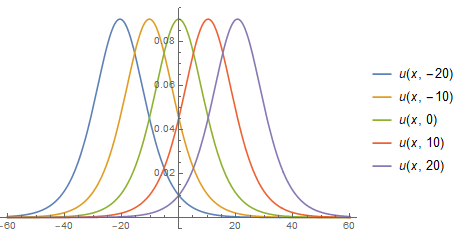
\includegraphics[width=8cm, height=5cm]{graf dcha.png}
  \caption{Representacion de la solución para distintos valores de t, para $c=103/100 \quad \beta=1 \quad \mbox{y} \quad z_{0} = 0$}
  \label{fig:despdch}
\end{figure}

\subsubsection{Caso 2:$c<\beta$ y $c<0$}

En este caso, para que $c-\beta$ y $c$ sean ambos negativos, debe cumplirse que $c<\beta$ y $c<0$. Esto implica que $c<0$, ya que $\beta$ es una constante real positiva. El signo de $c$ debe ser negativo, lo que nos indica que el solitón se desplazará hacia la izquierda conforme aumenta el tiempo con velocidad $c$. Ver Figura \ref{fig:despizq}.

\begin{figure}[h]
  \centering
    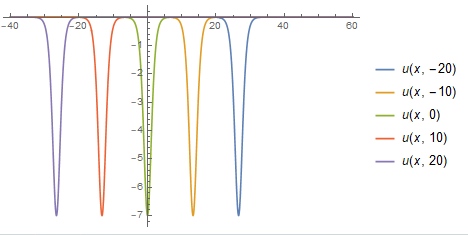
\includegraphics[width=8cm, height=5cm]{graf izq.png}
  \caption{Representacion de la solución para distintos valores de t, para $c=-103/100 \quad \beta=1 \quad \mbox{y} \quad z_{0} = 0$}
  \label{fig:despizq}
\end{figure}

\subsubsection{Caso 3: $c=\beta$}

En el caso límite, la amplitud seria $0$ por lo que $u(x,t)=0$ y se tiene una solución trivial.
% ----------------------------------------------------------------------

